\section{Interval Graph Recognition}

\subsection{Characterization}
Lekerkerker and Boland \cite{lekkerkerker1962representation} show that an undirected graph is an interval graph if and only if it is chordal and has no ATs. However, there are various other characterizations of interval graphs.

\begin{theorem}\cite{golumbic2004algorithmic}\cite{gilmore1964characterization}
Let G be an undirected graph. The following statements are equivalent.
\begin{enumerate}
\item $G$ is an interval graph.
\item $G$ is chordal and its complement $\bar{G}$ is a comparability graph.
\item The maximal cliques of G can be linearly ordered such that for every vertex $x$ of $G$, the maximal cliques containing $x$ occur consecutively.
\end{enumerate}
\end{theorem}



\subsection{Linear time Recognition algorithm}

The original linear time recognition algorithm of Booth and Lueker (1976)\cite{booth1976testing} is based on their complex PQ-tree data structure. R.M. McConnell and Y. Nussbaum(2009)\cite{mcconnell2009linear} demonstrate a linear time recognition algorithm using $\Delta$ modules for Probe Interval Graphs, which is a superclass of Interval Graphs. Habib et al.(2000) \cite{habib2000lex} show how to solve the problem more simply using lexicographic breadth-first search, based on the fact that a graph is an interval graph if and only if it is chordal and its complement is a comparability graph. A similar approach using a six-sweep LexBFS algorithm is described in Corneil, Olariu, and Stewart \cite{corneil2009lbfs}.

In this exam, we will focus on Booth and Leuker's recognition algorithm using the PQ-tree. Their algorithm has two steps. First, verify that G is a chordal graph, and enumerate its maximal cliques in $O(|V|+|E|)$ time. Second, test whether or not the cliques can be ordered so that those which contain vertex v occur consecutively for every $v \in V$. 

The number of maximal cliques will be at most $|V|$. This result will be proved by proposition \ref{num_max_clique}. 

\begin{proposition}
An arbitrary graph on $n$ vertices can have exponential maximal cliques.
\end{proposition}

\begin{figure}[H]
\centering
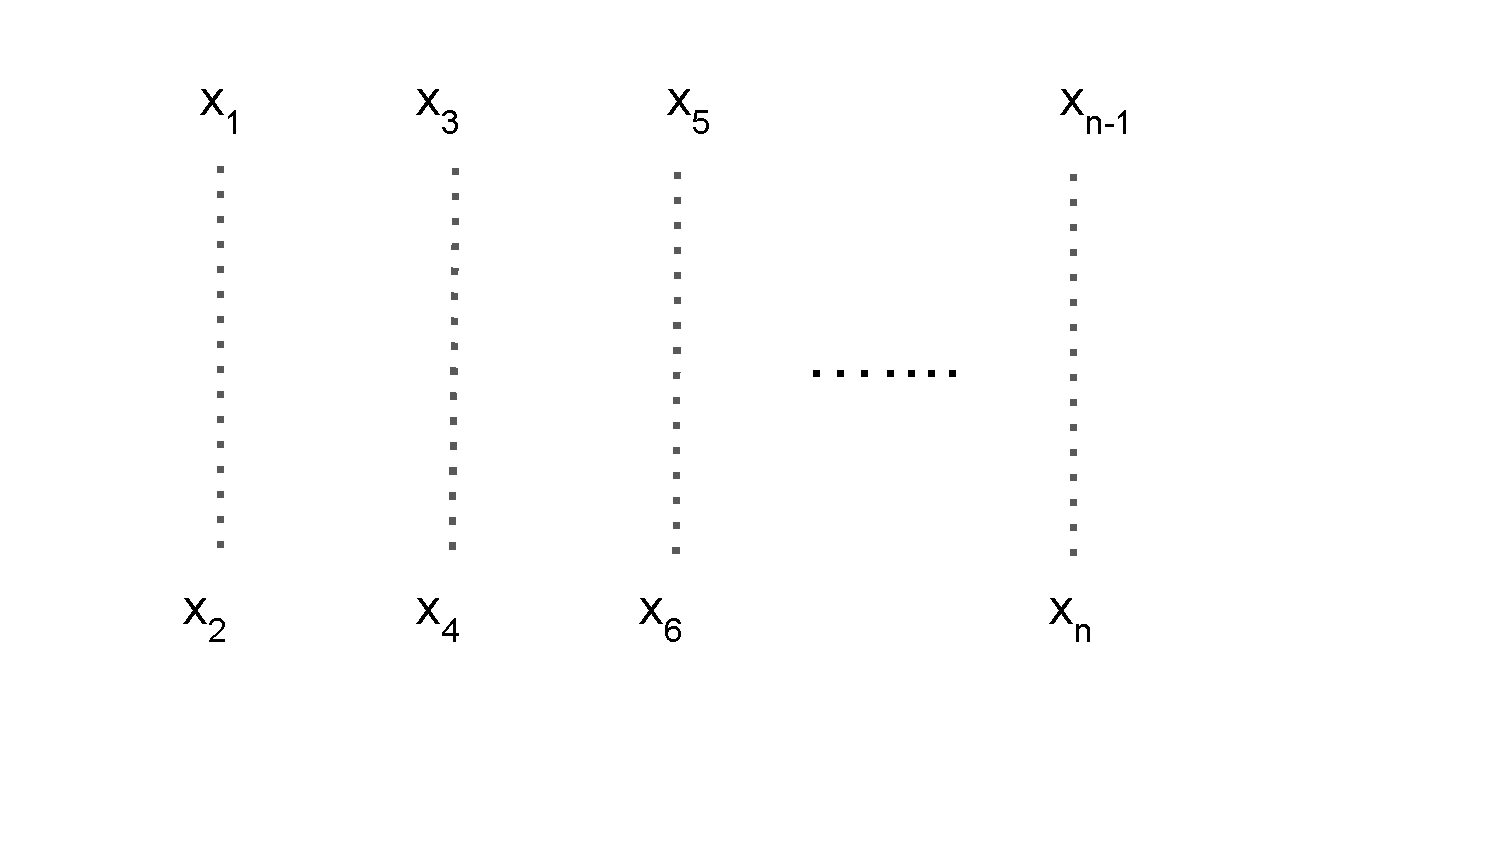
\includegraphics[width=8cm]{figures/recognition_1.pdf}
\caption{An example of a graph with exponential maximal cliques}
\label{recognition_1}
\end{figure}

\begin{proof}
In Figure \ref{recognition_1}, the vertical dotted lines denote the non-edges, all other pairs are edges. In this graph on n vertices, if we pick one vertex from each column, the set of vertices we select will always be a maximal clique. We have two choices in each column, thus, there are an exponential number of $2^{n/2}$ maximal cliques in this example graph.
\end{proof}

\begin{proposition}
\label{num_max_clique}
A chordal graph $G = (V, E)$ has at most $|V|$ maximal cliques, and we can find them in $O(|V|+|E|)$ time.
\end{proposition}

\begin{proof}
From each vertex $i$ in the perfect elimination ordering $\sigma$, $X_i = \{i\} \cup \{j \in Adj(i) |  \sigma^{-1}(j) > \sigma^{-1}(i) \} $ is a clique by definition of perfect elimination ordering. Any maximal clique $c$ is the same as $X_i$ if $i$ is the earliest vertex on $\sigma$. There are at most $|V|$ such $X_i$, so G has at most $|V|$ maximal cliques.

Not all $X_i$ are maximal cliques. We can easily modify Algorithm \ref{peo_test} without changing its running time, for line 13, if $A(v) = N(v)$, then $X_i$ is not a maximal clique, otherwise, it is maximal.
\end{proof}

\begin{figure}[H]
\centering
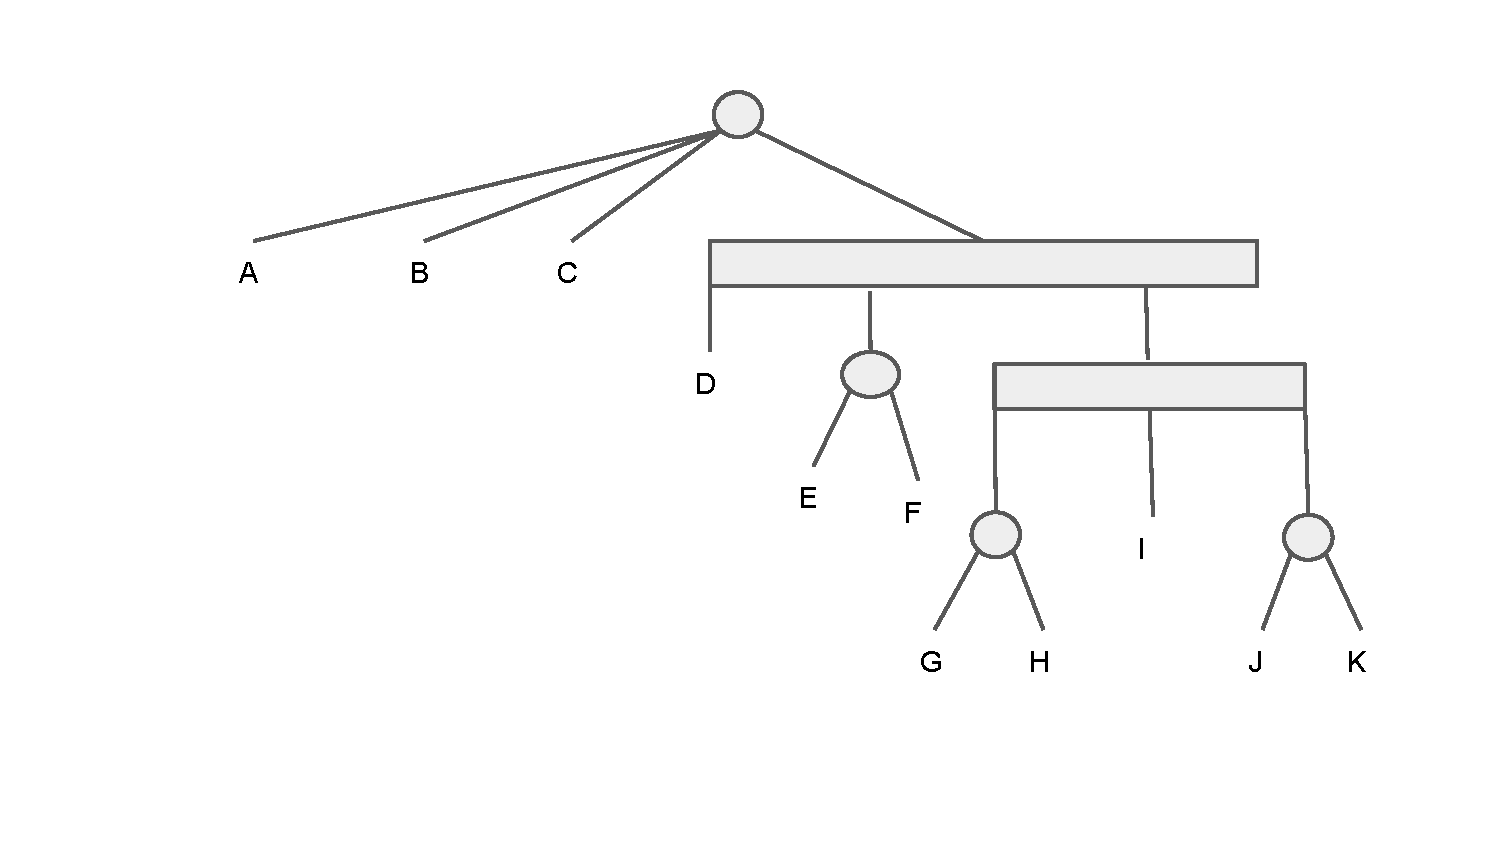
\includegraphics[width=12cm]{figures/pqtree_1.pdf}
\caption{A PQ-tree}
\label{pqtree_1}
\end{figure}

The PQ-tree data structure of is designed to represent a set of allowed permutations on its leaves. Its leaves form the set $X$ of maximal cliques of an interval graph. 
The $frontier$ of a tree T is the permutation of $X$ obtained by reading leaves' labels from left to right. The internal nodes have two types: type P and type Q. P nodes are usually denoted by circles and Q nodes by rectangles. A P node has at least two children and a Q node has at least three.
An \emph{equivalence transform} on a PQ-tree is one of the two operations below:

\begin{enumerate}
\item Arbitrarily permutes the order of the children of a P-node.
\item Reverse the order of the children of a Q-node.
\end{enumerate}

Two PQ-trees are equivalent by performing a series of equivalence transformation. Each transformation reorders the internal nodes of the tree and thus creates a new frontier. 

An example PQ-tree from Figure \ref{pqtree_1} has a frontier [A,B,C,D,E,F,G,H,I,J,K]. The PQ-tree in Figure \ref{pqtree_2} has a frontier [B,H,G,I,J,K,E,F,D,C,A]. It is not hard to see the two trees are equivalent by transformations. 

If two trees $T, T^{'}$ are equivalent, we denote $T \equiv T^{'}$. The set of all frontiers we obtained from trees equivalent to T is named \emph{consistent permutation} with $T$, and is denoted by $$CONSISTENT(T) = \{FRONTIER(T^{'})| T^{'} \equiv T \}$$

\begin{figure}[H]
\centering
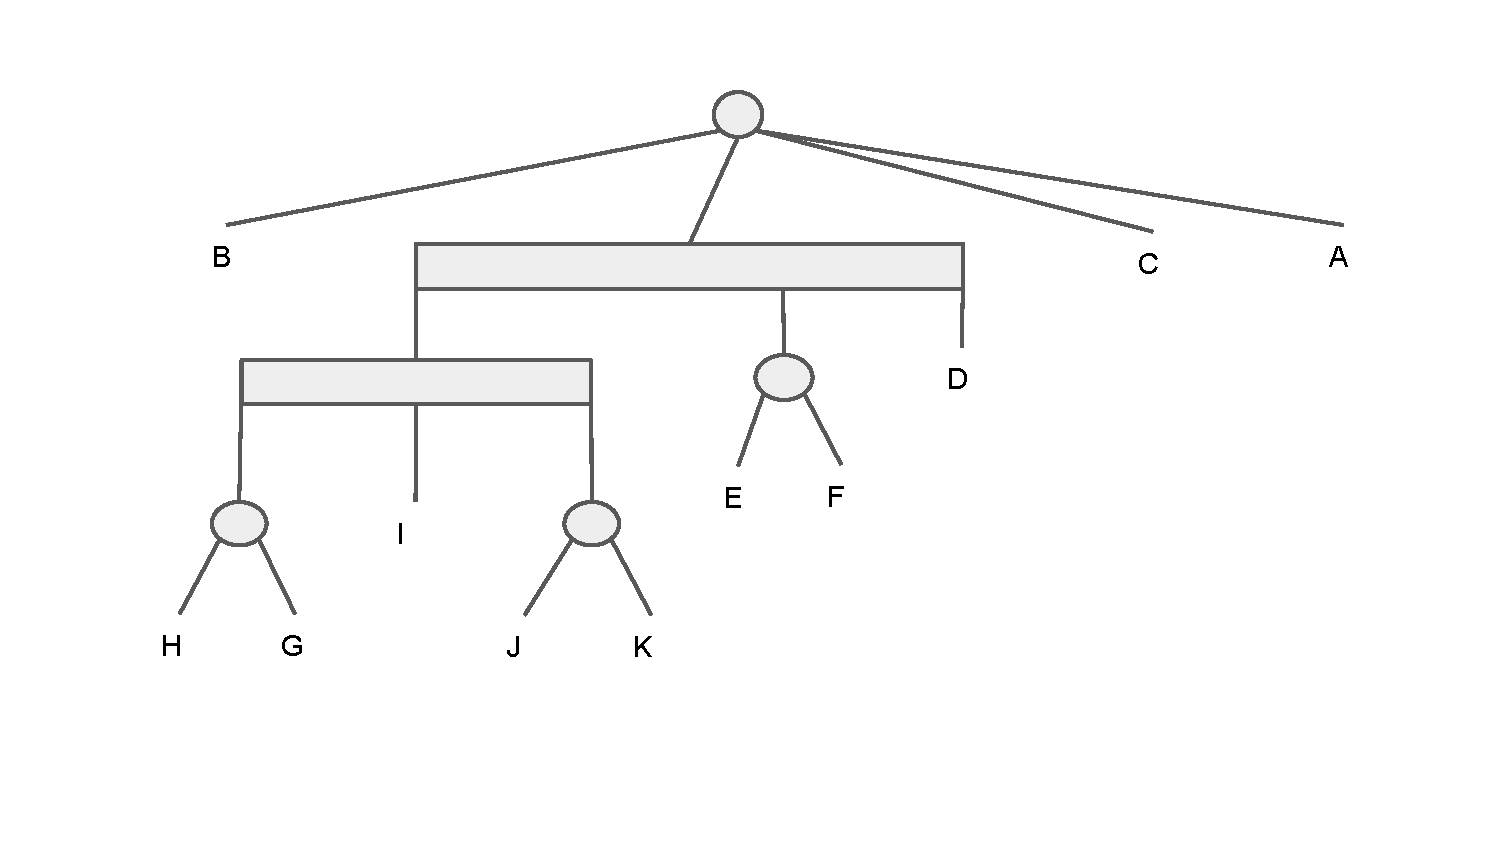
\includegraphics[width=12cm]{figures/pqtree_2.pdf}
\caption{An equivalent PQ-tree}
\label{pqtree_2}
\end{figure}

In the algorithm, there is only one operation called $Reduce(T,S)$. It returns the result PQ-tree after an S-reduction, which selects permutations from the consistent permutations of $T$ that is consecutive for a set $S \in U$. Figure \ref{pqtree_3} shows the tree in Figure \ref{pqtree_2} reduced by $S = \{ E,I,J,K\}$. The S-reduction is done by applying templates from bottom to the top. Each template is a pattern to match P or Q nodes and replace with a new structure. There are six templates for P nodes and three templates for Q nodes. To get the reductions done in Figure \ref{pqtree_3}, we need to apply template P3, Q3 (see Figure \ref{pqtree_p3q3}). For detailed explanation about other templates, the reader can go to Booth and Leuker's original paper\cite{booth1976testing}.

\begin{figure}[H]
\centering
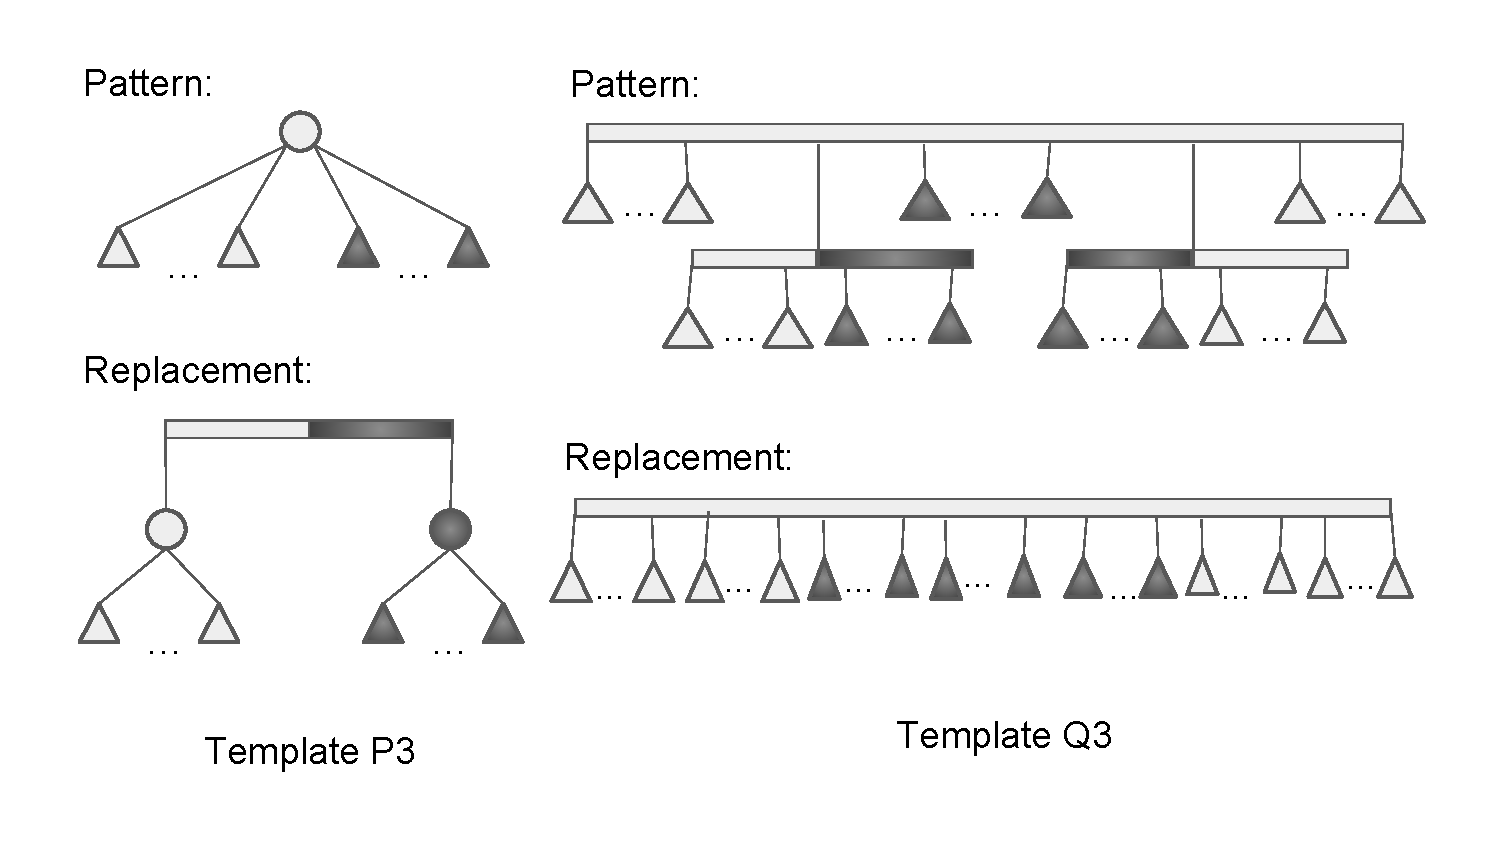
\includegraphics[width=16cm]{figures/pqtree_p3q3.pdf}
\caption{Template P3 and Q3}
\label{pqtree_p3q3}
\end{figure}


\begin{figure}[H]
\centering
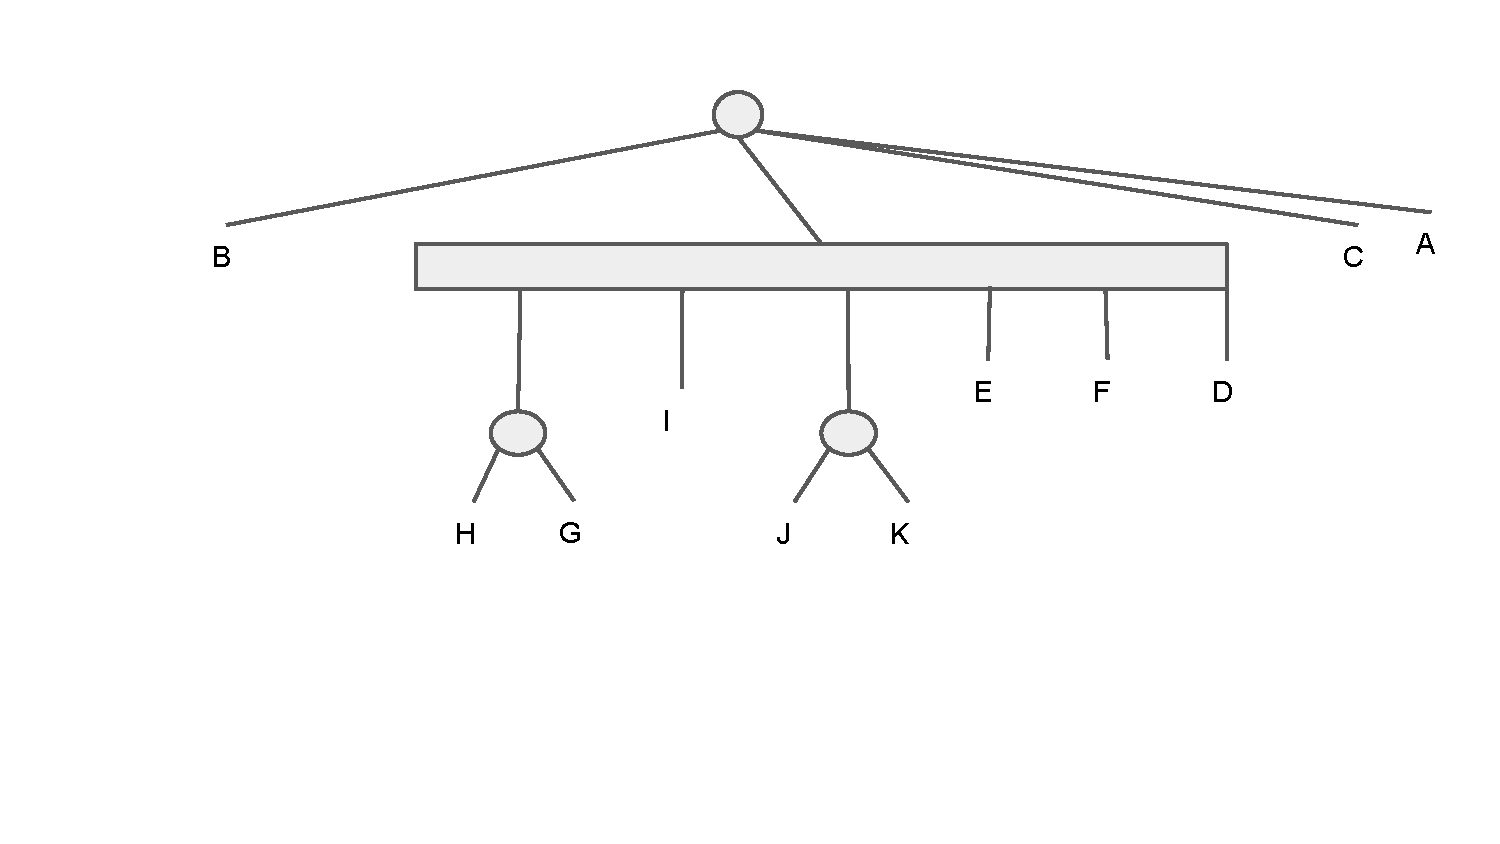
\includegraphics[width=12cm]{figures/pqtree_3.pdf}
\caption{A Reduced PQ-tree}
\label{pqtree_3}
\end{figure}

A \emph{universal tree} has only a P node which is the root and all members of $X$ are children of the root. Booth and Leuker's algorithm starts with a universal vertex $U$ of all maximal cliques, representing all possible permutations. Each time, a vertex $x$ is selected, and an S-reduction for the set of maximal cliques $S = \{C|x \in C\}$ is performed on this PQ-tree. The returned result is either an updated a PQ-tree or we find out it is impossible to get the consecutive-ones property for this vertex. Applying S-reductions for all vertices determines whether the consecutive-ones ordering is possible. If it is possible, the frontier of the final PQ-tree is a valid consecutive-ones ordering. An example of this procedure is in Figure \ref{pqtree_4}.

\begin{figure}[H]
\centering
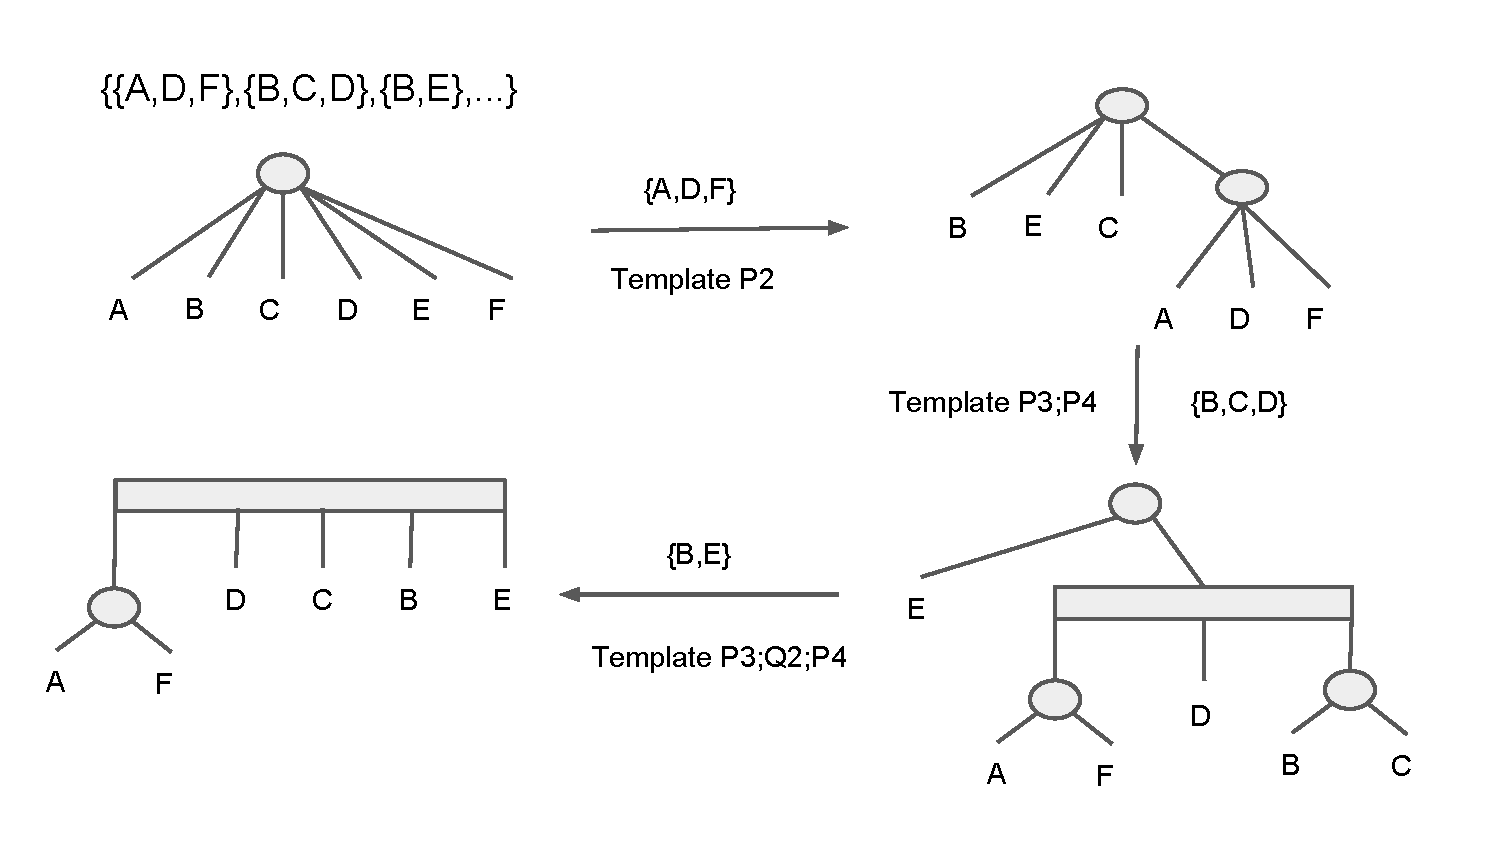
\includegraphics[width=12cm]{figures/pqtree_4.pdf}
\caption{An example of the procedures of reductions use templates Booth and Leuker\cite{booth1976testing}}
\label{pqtree_4}
\end{figure}

\begin{theorem}
\cite{booth1976testing}
If $M$ is an $m*n$ $(0,1)$-matrix specified by its $f$ nonzero entries, a consecutive-ones test can be performed in O(m + n + f) steps.
\end{theorem}




	












